\chapter{Literature Review}

\section{Introduction}

The purpose of this literature review is to synthesise and critically evaluate existing research relevant to the design of an Integrated Data Repository (IDR) and operational analytics dashboard aimed at improving post-MDT oncology pathway efficiency. Timely cancer treatment has profound implications for survival, patient experience, resource utilisation, and system performance. Evidence from national datasets, observational studies, systematic reviews, and informatics research shows that delays between MDT decisions and treatment initiation remain persistent across the NHS. Furthermore, data fragmentation, inconsistent recording practices, and limited visibility of operational bottlenecks hinder the ability of clinicians, MDT coordinators, and service managers to proactively manage these delays.

The review is organised around five interrelated themes:
\begin{enumerate}
    \item MDT operations and evolving pressures on multidisciplinary cancer decision making;
    \item Operational delays across the cancer pathway, particularly diagnosis-to-treatment intervals (DTI);
    \item Data fragmentation and the case for integrated data repositories;
    \item Dashboards and performance-monitoring tools to support operational decision-making;
    \item Emerging data trends and the role of ETL, interoperability, AI and multimodal data integration.
\end{enumerate}

Collectively, this literature forms the conceptual foundation (kernel theory) for the artefact developed in this study. The following sections provide a detailed account of these themes, integrating high-quality evidence from the UK, international datasets, clinical oncology, health informatics, and organisational science.

\subsection{Method}
An iterative literature review was adopted, following the guidance outlined by  \cite{dawson2015} (Figure \ref{fig:LitProc}). An initial search was conducted using Google Scholar and open-access repositories to identify foundationa concepts and terminology related to Integrated Data Repositories, cancer pathways, MDT operations, dashboards, and Design Science Research. These preliminary results infirmed a more structured search strategy applied to ScienceDirect, IEEEXplore, and PubMed.

Searches were limited to peer-reviewed journals, systematic reviews, national audits, and authoritative policy documents published primerily between 2010 and 2026, with earlier seminal works retained where conceptually relevant (e.g. Calman-Hine and Design Science Science foundations). Studies were included if they addressed MDT processes, oncology pathway delays, health data integration, dashboards, usability standards, or operational analytics. Articles focused exclusivly in molecular biology, single-modality clinical trials, or nomn-healthcare data systems were excluded. 

Appoximately 90 sources were reviewed during the processm with around 55 core studies retained for detailed analysis based on relevance, methodological quality, and applicability to NHS operational contexts. Backward citation tracking was used to identify influential seed papers and ensure conceptual completeness.

\begin{figure}
    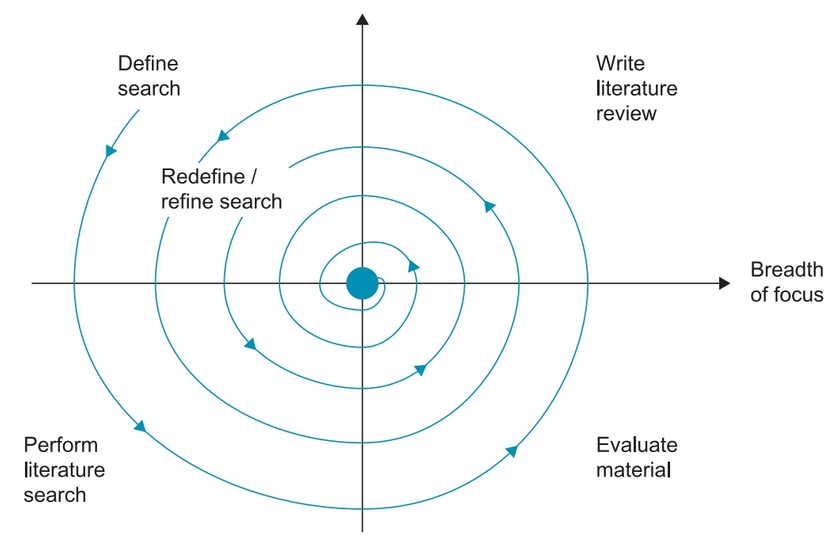
\includegraphics[width=\linewidth]{LitProc.png}
    \caption{Iterative literate review process \citep{dawson2015}}
    \label{fig:LitProc}
\end{figure}

\section{The NHS Cancer Pathway and MDT Framework}

\subsection{MDTs as the Backbone of UK Cancer Care}

Since the publication of the Calman–Hine report and subsequent interventions, MDTs have been embedded as the central governance structure for cancer decision making \citep{haward2006, price2014, morris2006, morris2008}. The MDT model mandates that every new cancer case in the UK is discussed by a multidisciplinary panel including oncologists, surgeons, radiologists, pathologists, specialist nurses, and allied professionals. The 2024 NHS Wales MDT Charter emphasises the crucial role MDTs play in standardising care, reducing unwarranted variation, and improving outcomes by bringing domain experts together in real time \citep{nhswales2024}. Prospective benefits include higher adherence to guidelines, improved communication, shared decision-making, and better coordination of multi-modal treatment plans.

However, the complexity of modern cancer care has increased dramatically alongside rising incidence, new treatment options, biomarker-based stratification, digital imaging volume, and genomic data availability. MDTs now contend with substantially larger case numbers, more complex diagnostic information, and resource pressures that stretch meeting capacity. Professional societies and national audits consistently highlight that MDT meetings are often over-subscribed, under-resourced, and administratively burdensome. These pressures compromise the quality of discussion and create operational bottlenecks that directly affect patient pathways.

\subsection{Evidence of MDT Operational Pressures}

Several studies provide evidence of the challenges affecting MDT functioning:

\begin{itemize}
    \item \cite{soukup2022} conducted a detailed observational analysis of 822 case discussions across three UK MDTs. Administrative and process issues occurred in 30\% of cases, attendance problems in 16\%, and equipment issues in 5\%. These logistical challenges significantly reduced the quality of information and decision-making, demonstrating how operational inefficiencies detract from MDT effectiveness.
    \item \cite{lim2025} analysed 1,488 UK HNC patients across 50 MDTs and found extremely low compliance with national cancer pathway standards: 32.8\% (FDS), 33.3\% (31‑day), and 34.6\% (62‑day). Median DTT-to-treatment was 42 days.
    \item \cite{chakravarty2023} demonstrated that patients referred from secondary-care outpatient pathways experienced significantly longer delays to MDT discussion and treatment (mean 102 vs. 88 days). These patients were also more likely to receive palliative rather than curative treatment.
    \item \cite{law2024} identified a decade of known MDT barriers including time pressures, communication challenges, inconsistent attendance, information deficits, and increasing clinical complexity.
\end{itemize}

While these studies consistently demonstrate operational strain within MDT processes, important limitations remain. Much of the evidence is observational and focuses primarily on decision quality or meeting efficiency rather than downstream operational consequences following MDT outcomes. Moreover, studies such as \cite{soukup2022} and \cite{law2024} emphasise human and organisational factors but do not address how data infrastructure or real-time operational visibility might mitigate these pressures. Large scale cohort analysis (e.g. \cite{lim2025}) quantify non-compliance with national standards but offer limited insights into the specific post-MDT workflow stages where delays emerge. As a result, although MDT pressures are well documented, the mechanisms by which MDT decisions translate into subsequent pathway delays remain poorly illuminated from an operational analytics perspective.  

\subsection{National policy direction and waiting time standards}

NHS England's 2024/25 planning guidance emphasises compliance with the Faster Diagnosis Standard (FDS) and cancer treatment timeliness metrics. Persistent waiting-time challenges, data-quality requirements, and the need for integrated pathway oversight tools are highlighted \citep{parker2026}. Radiotherapy services face particular strain: the Royal College of Radiologists reported over 2,300 breaches of the 31‑day standard in October 2023 \citep{rcr2024}. Hidden waits—such as 20‑week delays between surgery and radiotherapy—are not systematically captured, further illustrating limitations in operational visibility.

\section{Operational Delays in Cancer Pathways}

\subsection{Diagnosis-to-Treatment Interval (DTI) as a Critical Metric}

A robust body of literature demonstrates that prolonged DTI adversely affects survival across multiple cancer types.

Key findings include:

\begin{itemize}
    \item \cite{hanna2020}: A systematic review of 34 studies (1.27M patients) found each four-week delay increased mortality by up to 6–8\% across treatment modalities.
    \item \cite{coca-pelaz2018}: Delays in HNSCC beyond four weeks contribute to tumour progression and reduced local control.
    \item \cite{sharma2016}: Delays greater than 30 days reduce overall survival (HR 1.12), with mortality increasing 2.2\% per additional week.
    \item \cite{villemure-poliquin2025}: Treatment within 30 days improves survival by 9\%.
    \item \cite{saleh2024}: Cervical cancer survival drops dramatically after 30 days.
\end{itemize}

\subsection{Hospital/System Factors Influencing Delay}

Large-scale evidence shows that delays are driven not only by tumour characteristics but also by organisational inefficiencies:

\begin{itemize}
    \item \cite{yun2012}: Delays over one month worsened outcomes, especially in low-volume hospitals.
    \item UK audits (e.g., \cite{lim2025}) highlight delays in biopsies, imaging, scheduling, and treatment booking.
\end{itemize}

\subsection{MDT-specific drivers of post-decision delays}

\begin{itemize}
    \item Missing diagnostic information and administrative errors cause re-discussion delays \citep{soukup2022}.
    \item High caseloads reduce decision completeness.
    \item Secondary‑care referrals introduce additional diagnostic delays \citep{chakravarty2023}.
    \item Capacity constraints (radiotherapy, theatres, oncology clinics) generate downstream bottlenecks.
\end{itemize}

\subsection{Crititcal synthesis of delay literature}
Collectively, the literature provides compelling evidence that prolonged diagnosis-to-treatment intervals adversely affect survival accross multiple cancer types.. However, most studies treat delay as a single agregated interval rather than decomposing it into discrete operational stages. This limits their usefulness for operational improvement, as pathway delays arising from MDT decision latency, clinic availability, scheduling practices, or treatment capacity constraintsare rarely distinguished. Furthermore, while organisational factors such as hospital volume and service configuration are identified as contributors, few studies examine how real-time operational data could be leveraged to predict, prevent, or mitigate delays. This analytical gap constrains the translation of epidemiological evidence into actionable service-level interventions. 

\section{Data Fragmentation and the Need for Integrated Data Repositories}

\subsection{Fragmentation Across NHS Systems}

Oncology data spans EPRs, PAS, pathology, RIS/PACS, radiotherapy systems, chemotherapy e‑prescribing, Somerset/Cosmic, and MDT spreadsheets.

Evidence includes:

\begin{itemize}
    \item Operational policy from Royal Wolverhampton highlights inconsistent event definitions and PTL challenges \citep{theroyalwolverhamptonnhstrust2024}.
    \item \cite{varma2026}: 92.3\% agreement between CWT and hospital data only when treatment occurs within 100 days; discrepancies arise from definition mismatches and missing fields.
\end{itemize}

\subsection{Clinical Data Warehouses (CDWs) and the Evolution Toward IDRs}

Examples:

\begin{itemize}
    \item ROOT CDW: real‑time repository for 67,000+ cancer patients \citep{jung2021}.
    \item ONCO‑FAIR: chemotherapy‑specific FHIR extensions \citep{guilbert2024}.
    \item NHS–industry multimodal genomic-clinical data lake \citep{conway2025}.
    \item HN‑XNAT: federated imaging and radiotherapy repository \citep{butterworth2025}.
\end{itemize}

\subsection{Need for IDRs in NHS Operational Oncology}

Consequences of lacking IDRs include:

\begin{itemize}
    \item inability to track MDT→clinic→treatment transitions,
    \item inconsistent manual workarounds,
    \item reactive rather than proactive breach management,
    \item dependency on retrospective audits.
\end{itemize}

\section{Dashboards, Operational Analytics, and Decision-Support Systems}

\subsection{The Role of Dashboards in Performance Management}

Dashboards synthesise high-volume data for actionable insight. NHS guidance emphasises dashboards as essential for meeting FDS and treatment targets.

\cite{buttigieg2017} identify:

\begin{itemize}
    \item strategic dashboards,
    \item tactical dashboards,
    \item operational dashboards.
\end{itemize}

Key design principles include real‑time refresh, drill‑downs, user-centred design, and integration with data infrastructures.

\subsection{Clinical Decision-Support Dashboards and Multimodal Data}

Examples:

\begin{itemize}
    \item Multimodal CDSS supporting 170,000+ patients, using ETL + NLP + 140 data quality checks \citep{chang2025}.
    \item ROOT CDW: automated ingestion, structured/unstructured data integration \citep{jung2021}.
\end{itemize}

\subsection{Data Quality and Informatics Challenges}

Dashboards depend on strong data foundations:

\begin{itemize}
    \item Coding variation limits dataset reliability \citep{varma2026}.
    \item Oncology workloads require custom FHIR extensions \citep{guilbert2024}.
    \item Multimodal data lakes require governance and standardisation \citep{conway2025}.
\end{itemize}

\section{Usability, HCI, and ISO 9241‑110}

ISO 9241‑110:2020 \citep{internationalorganizationforstandardization2020} provides seven principles:

\begin{enumerate}
    \item Suitability for the task
    \item Self-descriptiveness
    \item Conformity with user expectations
    \item Learnability
    \item Controllability
    \item Error tolerance
    \item Suitability for individualisation
\end{enumerate}

Fraunhofer usability research supports its relevance in healthcare \citep{hunkirchen}.

\section{AI‑Enabled MDT Systems and Emerging Technologies}

Examples include:

\begin{itemize}
    \item EvoMDT: multi-agent MDT recommender reducing decision time by 30–40\% \citep{liu2026}.
    \item TrustedMDT: TNM staging and guideline checking integrated with Teams \citep{soltan2025}.
    \item AI‑MDT for lung cancer: improved throughput and workload reduction \citep{liu2026a}.
    \item AI automation of transcription and summarisation \citep{healthorbit2025}.
    \item Multi-agent consensus MDT system achieving high inter-agent agreement \citep{han2025}.
\end{itemize}

A key insight: AI systems require structured, linked, high‑quality data—yet most NHS operational systems lack it.

\section{Synthesis of Gaps}

The reviewed literature reveals several interlocking gaps that collectively motivate this research. First, despite clear evidence of clinically significant delays between MDT decision and treatment initiation, NHS oncology services lack granular, operationally focused visibility of post-MDT pathway stages. Second, although dashboards are widely promoted as performance management tools, many NHS implementations remain dependent on retrospective, aggregate reporting derived from fragmented and inconsistently defined datasets. As a result, existing dashboards often identify breaches only after they have occurred, limiting their utility for proactive intervention.
Third, while clinical data warehouses and integrated repositories have demonstrated feasibility in research and tertiary settings, their designs typically prioritise longitudinal research use cases rather than real-time operational decision-making. Consequently, issues of event harmonisation, timeliness, and alignment with national cancer waiting time definitions remain unresolved in day-to-day service management. Finally, emerging AI-enabled MDT systems highlight future opportunities for decision automation but simultaneously expose a foundational dependency on structured, integrated, and operationally reliable data infrastructures that are currently absent in most NHS Trusts.
Together, these gaps indicate the need for an artefact that integrates operational oncology data across MDT, clinic, and treatment domains, and presents this information through a user-centred dashboard explicitly designed to support proactive post-MDT workflow management.

\begin{itemize}
    \item \textbf{Gap 1} — Lack of integrated operational visibility
    \item \textbf{Gap 2} — Significant treatment delays persist
    \item \textbf{Gap 3} — Siloed systems hinder analytics
    \item \textbf{Gap 4} — Dashboard capability depends on ETL and interoperability
    \item \textbf{Gap 5} — No integrated framework across MDT, IDR, dashboards, usability
    \item \textbf{Gap 6} — AI MDT systems require structured data not currently available
\end{itemize}

\section{Summary}

This literature review synthesises evidence across MDT functioning, treatment delays, operational workflow challenges, data fragmentation, health informatics, dashboard design, usability standards, and emerging AI-driven MDT tools. MDTs remain vital but increasingly pressured. Delays between diagnosis, MDT decisions, and treatment initiation significantly worsen outcomes, yet Trusts lack the integrated systems required to manage these pathways proactively. Modern CDWs demonstrate feasible architectures, while dashboard and usability literature highlight design imperatives. AI‑enabled MDT systems reveal future potential but highlight the foundational need for high-quality integrated data repositories.

The combined evidence exposes a clear research gap: NHS oncology services require a robust, user-centred, IDR‑backed operational dashboard to improve MDT‑to‑treatment coordination.